%When the theory of the electroweak interaction was first developed \cite{1959.Glashow.vector-mesons, 1959.Salam.electroweak},
%the $W$ and $Z$ bosons were predicted to be massless (a typical mass term in the Lagrangian would violate the SU(2) symmetry).
%However, these were experimentally observed to have masses...

The results of electroweak mixing and the implications of the Higgs field have been introduced in the previous section.
If the EWK theory were an unbroken symmetry, the associated $W^{\pm}$ and $Z$ bosons would be massless; however, when observed experimentally, they were found to be quite heavy~\cite{1983.w-boson, 1983.z-boson}, at around $80\gev$ and $91\gev$, respectively~\cite{2014.pdg}.
Here, a more detailed explanation of the Higgs mechanism and how it ``spontaneously breaks'' the EWK symmetry, resulting in the three massive bosons ($W^\pm$ and $Z$) and one massless boson (photon), is presented.

To see how the Higgs mechanism results in the massive vector bosons and a massless photon, consider the following.
Beginning with a complex scalar doublet $\phi$ defined as:
\begin{equation}
  \phi = 
  \begin{pmatrix}
    \phi^{+} \\
    \phi^{0}
  \end{pmatrix}
  = \sqrt{\frac{1}{2}}
  \begin{pmatrix}
    \phi_1 + i\phi_2 \\
    \phi_3 + i\phi_4
  \end{pmatrix}
  \label{eq:complex_scalar_doublet}
\end{equation}
a Lagrangian $\mathcal{L}$ can be written:
\begin{equation}
  \mathcal{L} = (\mathcal{D}_\mu\phi)^\dagger (\mathcal{D}^\mu\phi) - \mu^2\phi^{\dagger}\phi-\lambda (\phi^{\dagger}\phi)^2
  \label{eq:complex_scalar_lagrangian}
\end{equation}
where $\lambda > 0$ and $\mathcal{D}_{\mu}$ is the covariant derivative.
$\mathcal{D}_\mu$ is defined such that $\mathcal{L}$ is invariant under a local $\gtsu{2}\times\gtu{1}$ gauge transformation:
\begin{equation}
  \mathcal{D}_{\mu}\phi = \bigg(\partial_{\mu} + \frac{ig}{2}\tau_a W_{\mu}^a + \frac{ig'}{2}B_{\mu}\bigg)\phi
  \label{eq:covariant_deriv}
\end{equation}
where $W_{\mu}^a$ ($a=1,2,3$) are the $\gtsu{2}$ fields with generators $\tau_a$ and coupling constant $g$, and $B_{\mu}$ is the $\gtu{1}$ field with coupling constant $g'$.

Isolating the potential term:
\begin{equation}
  V(\phi) = \mu^2\phi^{\dagger}\phi+\lambda(\phi^{\dagger}\phi)^2
  \label{eq:higgs_potential}
\end{equation}
a choice must be made on the sign of $\mu^2$, and the case of interest is for $\mu^2 < 0$. % \TODO{page 328, 334}
This results in the famous ``mexican hat potential'' shown in Figure~\ref{fig:mexican_hat}, which is minimized along the collection of points:
\begin{equation}
  \phi^{\dagger}\phi = \frac{1}{2}\big(\phi_1^2 + \phi_2^2 + \phi_3^2 + \phi_4^2\big) = -\frac{\mu^2}{2\lambda}
  \label{eq:higgs_minimum}
\end{equation}
This means that the minimum of the potential is not at $\phi = 0$ (as it would be in the case where $\mu^2 > 0$), but rather at a value:
\begin{equation}
  v \equiv \sqrt{-\frac{\mu^2}{\lambda}}
  \label{eq:higgs_minimum_value}
\end{equation}
With no loss of generality due to the $\gtsu{2}$ symmetry, $\phi_1 = \phi_2 = \phi_4 = 0$ can be set in Equation~\ref{eq:higgs_minimum} leaving $\phi_3^2 = v^2$.
Finally, the \emph{vacuum expectation value} (VEV) of the field can be written as:
\begin{equation}
  \langle\phi\rangle = \sqrt{\frac{1}{2}}
  \begin{pmatrix}
  0 \\ v
  \end{pmatrix}
  \label{eq:vev}
\end{equation}

\begin{figure}[htbp]
  \centering
  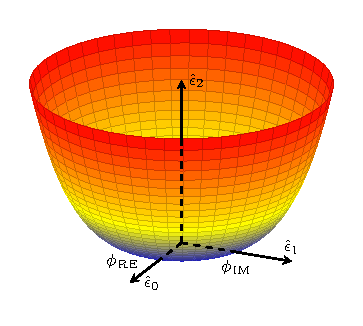
\includegraphics[width=.48\textwidth]{figs/theory/higgspotential_greater0}
  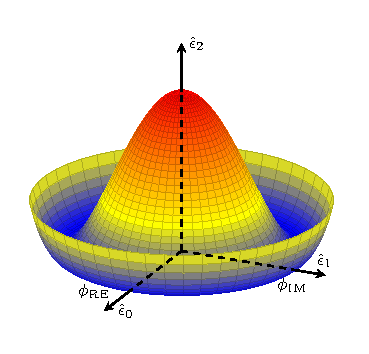
\includegraphics[width=.48\textwidth]{figs/theory/higgspotential}
  \caption{An illustration of the potential term $V(\phi)$ in the cases where $\mu^2 > 0$ (left) and $\mu^2 < 0$ (right).  The right-hand plot shows the Higgs potential, or ``Mexican hat potential'', with the minimum at $|\phi| = \sqrt{-\frac{\mu^2}{\lambda}}$ rather than at $|\phi| = 0$ as in the left-hand plot.}
  \label{fig:mexican_hat}
\end{figure}

The VEV can be substituted back into the original Lagrangian in Equation~\ref{eq:complex_scalar_lagrangian}, and, following quite a bit of math, a collection of mass terms can be identified:
\begin{equation}
  \mathcal{L} \subset \mathcal{L}_M \equiv \frac{1}{8}v^{2}g^{2}\bigg[\big(W_{\mu}^1\big)^2 + \big(W_{\mu}^2\big)^2\bigg] + \frac{1}{8}v^2\bigg[g^{2}\big(W_{\mu}^3\big)^2 - 2gg'W_{\mu}^{3}B^{\mu} + g'^{2}\big(B_{\mu}\big)^{2}\bigg]
  \label{eq:higgs_mass_1}
\end{equation}
Focusing on the first term for the moment, substituting in Equation~\ref{eq:w_mixing} for the physical $W^\pm$ bosons, the mass term can be seen clearly:
\begin{equation}
  M_W^{2}W^{+}W^{-} = \bigg(\frac{1}{2}vg\bigg)^{2}W^{+}W^{-}
\end{equation}
\begin{equation}
  M_W = \frac{1}{2}vg
\end{equation}
With a bit of clever forward-thinking, the second term of Equation~\ref{eq:higgs_mass_1} can be rewritten as:
\begin{equation}
  \frac{1}{8}v^{2}\bigg[gW_{\mu}^{3} - g'B_{\mu}\bigg]^2 + 0\bigg[g'W_{\mu}^{3} - gB_{\mu}\bigg]^2 =  \frac{1}{2}M_{Z}^{2}Z_{\mu}^{2} + \frac{1}{2}M_{A}^{2}A_{\mu}^{2}
  \label{eq:higgs_mass_2}
\end{equation}
where $Z_{\mu}^{2}$ and $A_{\mu}^2$ represent the physical $Z$ boson and photon, respectively, and are defined as:
\begin{equation}
 Z_{\mu} = \frac{gW_{\mu}^{3} - g'B_{\mu}}{\sqrt{g^2+g'^2}}
  \label{eq:higgs_z}
\end{equation}
\begin{equation}
  A_{\mu} = \frac{g'W_{\mu}^{3} - gB_{\mu}}{\sqrt{g^2+g'^2}}
  \label{eq:higgs_a}
\end{equation}
From this, it can be seen that the photon is massless, and the mass of the $Z$ boson is identified as:
\begin{equation}
  M_Z = \frac{1}{2}v\sqrt{g^2+g'^2}
\end{equation}

Lastly, the Higgs field can couple directly to the fermions.
Taking the electron as an example, an additonal Lagrangian term can be written:
\begin{equation}
\mathcal{L}_e = -G_e \big[\bar{e}_{L}\phi e_R+\bar{e}_R\phi^{\dagger}e_L\big]
\end{equation}
where $e_L$ and $e_R$ are the left-handed doublet and right-handed singlet, respectively, and $\phi$ is as in Equation~\ref{eq:complex_scalar_doublet}.
The symmetry can be spontaneously broken by a perturbation about the VEV:
\begin{equation}
  \phi = \sqrt{\frac{1}{2}}
  \begin{pmatrix}
  0 \\ v+h(x)
  \end{pmatrix}
\end{equation}
which, when substituted into $\mathcal{L}_e$ gives:
\begin{equation}
  \begin{aligned}
    \mathcal{L}_e &= -\frac{G_e}{\sqrt{2}}v\big(\bar{e}_{L}e_{R}+\bar{e}_{R}e_{L}\big) - \frac{G_e}{\sqrt{2}}\big(\bar{e}_{L}e_{R}+\bar{e}_{R}e_{L}\big)h \\
                  &= -m_e\bar{e}e-\frac{m_e}{v}\bar{e}eh
  \end{aligned}
\end{equation}
for electron mass $m_e = \frac{G_{e}v}{\sqrt{2}}$.
From the second term, it can be seen that the strength of the Higgs coupling to the electron is proportional to the mass of the electron.
The rest of the fermion couplings follow from this example.

What is accomplished here is quite remarkable.
The weak and electromagnetic interactions have been unified into a single $\gtsu{2}\times\gtu{1}$ interaction, and the physical bosons observed in nature arise as mixtures of the four gauge fields.
Additionally, the non-zero VEV of the Higgs field results in masses for the $W^{\pm}$ and $Z$ bosons while the photon remains massless.
Additionally, it is shown that the Higgs couples to fermions in proportion to their mass.
From experimental measurements, the value of the VEV has been determined to be $v\approx 246\gev$~\cite{2014.pdg}.
However, it should be noted that the theory does not predict the mass of the Higgs boson or of the fermions; these must all be determined from experiment.
